%
% ---------- header -----------------------------------------------------------
%
% project       kaneton
%
% license       kaneton
%
% file          /home/mycure/kaneton/view/book/kaneton/background.tex
%
% created       julien quintard   [tue jun 19 11:48:36 2007]
% updated       julien quintard   [wed dec 19 15:47:51 2007]
%

%
% ---------- background -------------------------------------------------------
%

\chapter{Background}
\label{chapter:background}

This chapter introduces some notions about operating systems and kernels.
However, this chapter assumes the reader already has a substential knowledge
about operating systems internals.

\newpage

%
% ---------- text -------------------------------------------------------------
%

%
% distributed operating system
%

\section{Distributed Operating System}

To understand the kaneton microkernel design and implementation, the reader
must first understand what are the distributed operating systems requirements
and more generally what are distributed systems inherent problems.

A distributed operating system can be defined through different ways and
the reader should probably find different definitions in the literature. In
this document, we assume that the main goal of a distributed operating
system is to connect users and resources in a transparent, open, and scalable
way.

For instance, when a user launches a program, the distributed operating system
decides on which machine of the network to run it. More generally, for
any action to perform, the distributed operating system tries to find the
most suitable place for executing it depending on resources availability.

While the processes generally communicate with each other on the same
machine, in a distributed operating system, they also communicate with the
other processes of other machines as illustrated in \textit{Figure
\ref{figure:distributed-operating-system}}.

\begin{figure}[h]
  \begin{center}
    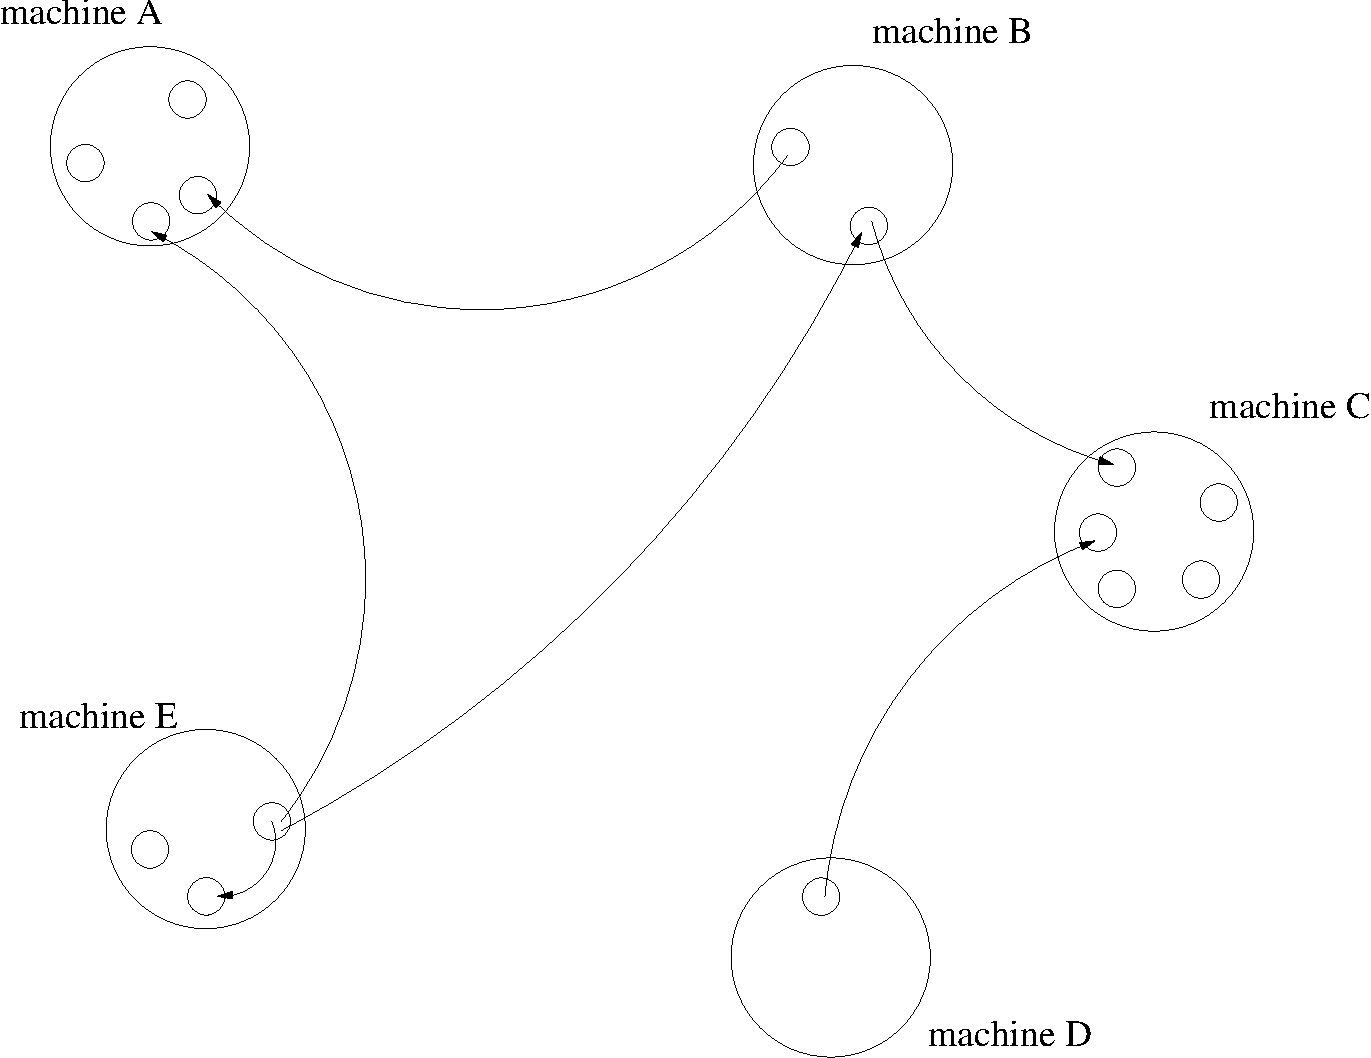
\includegraphics[scale=0.5]{\path/figures/distributed-operating-system.pdf}
    \caption{Communications in a distributed operating system.}
    \label{figure:distributed-operating-system}
  \end{center}
\end{figure}

In \textit{Figure \ref{figure:distributed-operating-system}}, the machine
named \textit{E} is running three processes. One is just running some
computations performing no communication, another is receiving a message
from the latter which is also sending two messages to processes over the
network.

These communications can be simple point-to-point communication for example
between a client and a web server while other can be distributed operating
system specific messages intended to make decisions on the location of a file
on the distributed file system for instance.

We saw that machines on a distributed operating system are running processes
which communicate with any other processes of any other node. Every machine
needs an operating system to organize the computer resources and to make
them communicate.

Microkernel-based operating systems are the best suitable systems
for building a distributed operating system as these systems are modular
and reliable by nature.

%
% microkernel
%

\section{Microkernel}

A microkernel is a kernel type designed to be modular hence more reliable than
monolithic kernels. Instead of building a large binary object containing the
kernel itself, the drivers, the file systems etc. microkernels try to be as
small as possible, providing only the fundamental services for managing
memory, execution contexts, communication and input/output. Besides, the other
classical operating system services are provided by userland processes with
special privileges.

This very specific design is very interesting for security, maintainability
and extensibility. Moreover, this type of design perfectly fits
distributed operating systems requirements where special processes
communicate with other node's processes to organize the whole distributed
system resources.

Figure \ref{figure:microkernel} illustrates a microkernel view with different
layers.

\begin{figure}[h]
  \begin{center}
    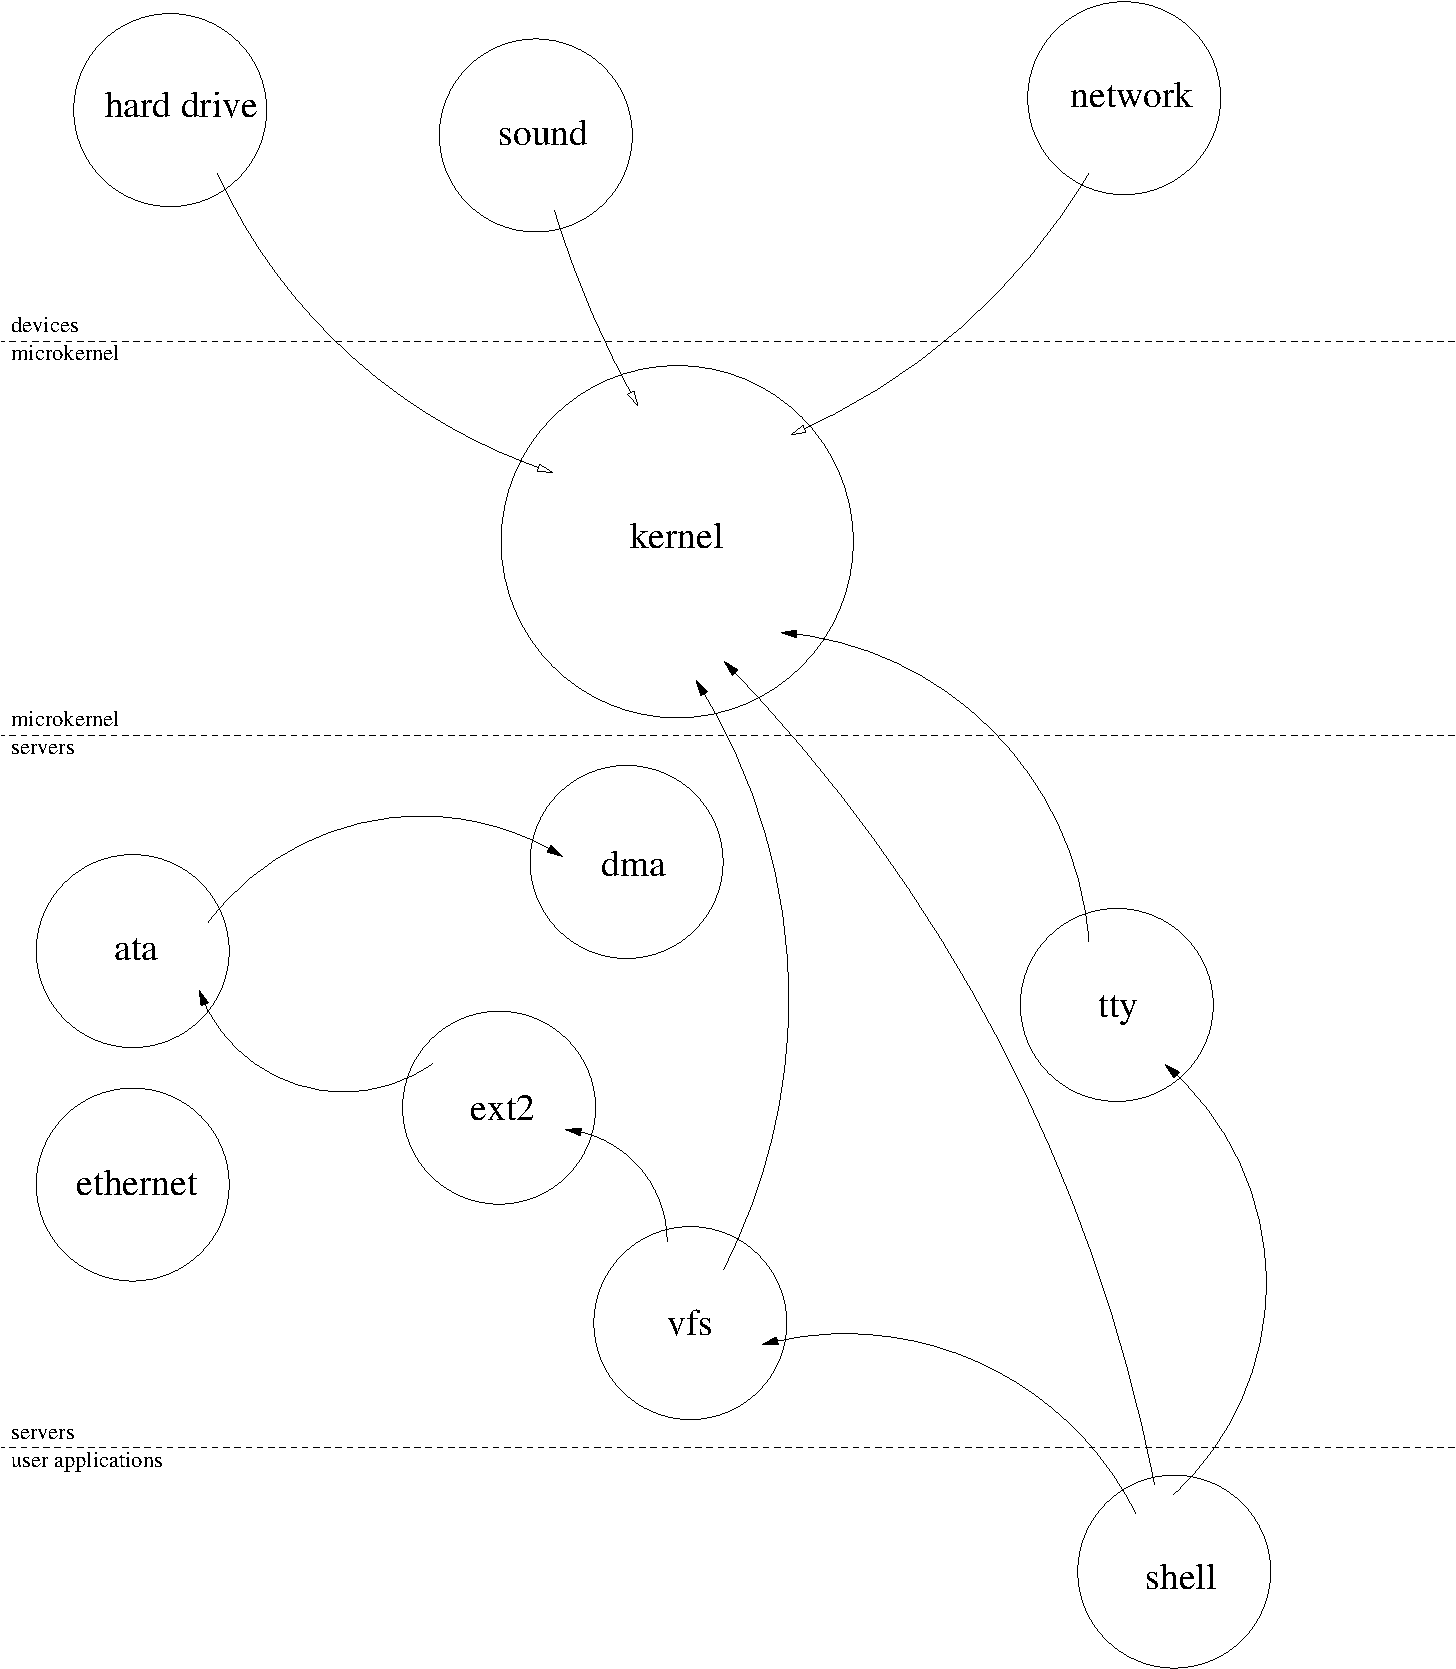
\includegraphics[scale=0.4]{\path/figures/microkernel-behaviour.pdf}
    \caption{Communications in a microkernel hierarchy.}
    \label{figure:microkernel}
  \end{center}
\end{figure}

The whole microkernel design is based on the client-server communication
model where clients ask servers to perform a specific task. For instance,
to print some text to the screen, a user program has to ask the \textit{tty}
server to do it for him because the user program itself does not have any
right to perform such an action.

To avoid complications and deadlocks the microkernel follows a fundamental
rule which restrict communication from clients only to more or equal
privileged tasks. On the Figure \ref{figure:microkernel}, the \textit{vfs}
server can ask the \textit{ata} server and the \textit{kernel} to peform a
task but the kernel cannot ask a less privileged server to do something for
him.
